\section{Experiments and Results}
\label{sec:experiments}
\subsection{Design and reproducibility}
These experiments evaluate the current website engine under stated assumptions, rather than calibrating it to field observations. We compare lower-demand arrival rates of 40 and 30 people/minute at entries A and B with the defaults of 120 and 80. Each baseline is run with and without a surge adding 60 people/minute to \emph{each} entry during minutes 0--10. Each of the four scenarios has 30 independently seeded, empty-start, 40-minute trajectories. States are recorded every five seconds; events between observations are still processed at their scheduled times.

Fixed parameters are four lifts per bank, capacity limit 20, mean cycles 40 and 200 seconds, cycle standard deviations 4 and 20 seconds, speed 1.3 m/s, spacing 0.45 m/person and Logit sensitivity $\beta=0.05\,\mathrm{s}^{-1}$. Trip capacity uses the implemented discrete distribution on 16--20, with mean 18. Cycle draws are truncated below ten seconds. The queue-length walking rule is used, rather than the optional mapped-route rule.

The primary outcome is the number not boarded by minute 40, including people queueing and walking. We also record arrivals, boarding fraction and mean arrival-to-boarding time among completed passengers. The latter excludes unfinished waits and is not the mean for all arrivals. Intervals use independent trajectory outcomes, $\bar{x}\pm t_{29,.975}s/\sqrt{30}$; within-run snapshots are not treated as independent replications.

\subsection{Demand and finite-horizon backlog}
The approximate nominal total service rate is
\[
\mu_{\rm total}=60\left(\frac{4\times18}{40}+\frac{4\times18}{200}\right)
=129.6\ \text{people/minute}.
\]
The default baseline of 200 therefore exceeds nominal service before any surge; 70 leaves recovery capacity after the surge ends. The ten-minute surge adds an expected 1,200 entrants across the two entries.

\begin{center}\small
\begin{tabular}{@{}lrrrr@{}}
\toprule
Baseline & Surge & Arrivals & Not boarded at 40 min & Boarded delay (s)\\
\midrule
70/min & No & 2,805.7 & $16.4\pm3.6$ & 14.3\\
70/min & Yes & 3,999.8 & $15.1\pm3.7$ & 102.9\\
200/min & No & 7,985.2 & $2,816.5\pm33.7$ & 402.6\\
200/min & Yes & 9,205.3 & $4,028.5\pm41.7$ & 609.2\\
\bottomrule
\end{tabular}
\captionof{table}{Means over 30 trajectories. The $\pm$ entries are 95\% t-interval half-widths for final backlog only. Delay includes only passengers boarded before the horizon.}
\end{center}
\begin{center}
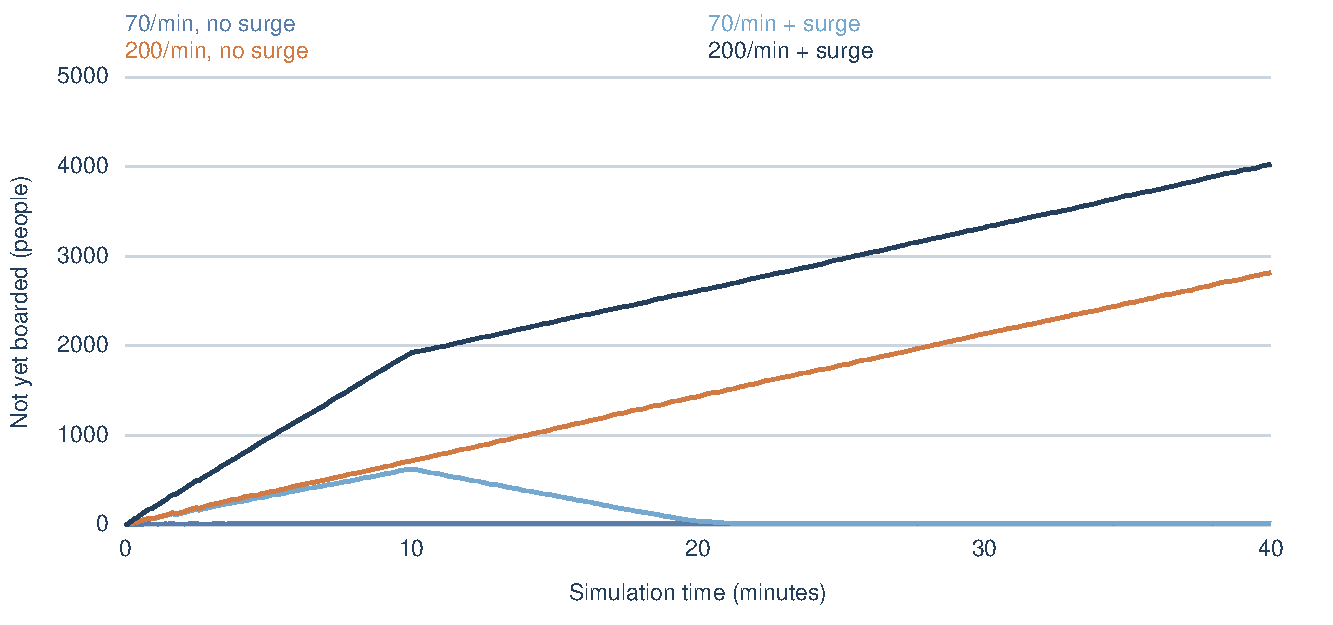
\includegraphics[width=.9\linewidth,height=7cm,keepaspectratio]{figures/backlog_traces.pdf}
\captionof{figure}{Mean number not yet boarded, including queued and walking passengers. All scenarios start empty.}
\end{center}

\newpage
\subsection{Interpretation and conditional-table checks}
At lower baseline demand, the surge raises completed-passenger mean delay from 14.3 to 102.9 seconds, but final backlog remains approximately 15--16 people. The trajectory plot shows recovery within the horizon. Similar final counts do not imply equal experience: substantial delay can occur before the system clears.

At default demand, accumulation persists without a surge. Adding the surge raises final backlog from 2,816.5 to 4,028.5 people, while mean boarding fraction falls from 64.7\% to 56.2\%. Around 5,170 people board in either default-demand scenario, consistent with a service-limited system. Redistributing choices cannot offset sustained total inflow above total service. These results do not measure a real-world benefit of recommendations: no alternative recommendation or adoption policy has been compared.

\paragraph{Conditional distribution collection.}
A separate default-plus-surge collection recorded exactly 1,000,000 paired queue snapshots over 2,084 independently seeded trajectories, including a partial final trajectory. Sampling is every five seconds with five-minute bins. There are 7,400 entry/window/local-count cells; 5,666 have at least 30 matches. Cell counts across both entry views sum to 2,000,000 because each joint observation contributes once per view, not because it represents two independent observations. Histogram counts exactly match each cell's count, and accumulated costs are finite.

The lookup estimates
\[
\widehat{P}(N_{\rm other}=k\mid E=e,W=w,N_{\rm local}=m)
=\frac{h_{e,w,m}(k)}{n_{e,w,m}},
\]
where $h$ is the matching histogram and $n$ its total. Conditional expected costs are stored cost sums divided by $n$. Histogram quantiles describe simulated variability, not confidence intervals. Thirty matches is a display safeguard, not a statistical guarantee. The table is generated under full-information choice behaviour, so it supports an occasional lookup user under that generating regime. Mass adoption changes behaviour and requires new policy simulations.

\paragraph{Implementation verification and limits.}
Model and API checks passed for NHPP integrals and pulse boundaries, stable Logit behaviour, position-loss costs, seeded reproducibility, conservation including walkers, capacities, conditional aggregation, transport parity and invalid requests. All 120 experimental trajectories satisfy arrivals equal the sum of boarded, queued and walking passengers at the horizon. These checks establish implementation consistency, not empirical validity or agreement with a separate SimPy implementation.

Results remain conditional on uncalibrated arrival, service and behavioural assumptions. High-demand states stretch the walking rule: spacing times combined queue length can imply distances much longer than the corridor. The actual engine serves passengers during their walk, while perceived cost uses a current-rate approximation and excludes existing walkers from observed queue lengths. Empty starts, a single surge and finite-horizon censoring further restrict generalisation. These results are stress experiments and should remain distinct from subsequently calibrated team results.
